\chapter{Aspekt techniczny systemu}
Poniższa część pracy skupia się na aspekcie technicznym tworzonego systemu.
Dzięki przygotowanej w poprzednim rozdziale wizji aplikacji, możliwe jest
skupienie się teraz na konkretnej implementacji. Przedstawione zostaną aspekty
takie jak wybór technologii i architektura systemu. Opisany zostanie również
proces implementacji i testowania.

\section{Technologia implementacji}
W dzisiejszym dynamicznym środowisku technologicznym, tworzenie aplikacji
mobilnych stanowi zadanie wymagające przemyślanego podejścia do wyboru
odpowiednich technologii. Wraz z różnorodnością dostępnych platform, języków
programowania oraz narzędzi deweloperskich, napotykamy szeroki zakres możliwości
i wyzwań podczas decydowania, jak zrealizować wizję aplikacji mobilnej. W miarę
jak branża ewoluuje, zauważalne są rozbieżności pomiędzy różnymi technologiami,
a także ich wpływ na wydajność, dostępność oraz doświadczenia użytkownika. Od
natywnych aplikacji po rozwiązania hybrydowe i progresywne, każda opcja posiada
swoje unikalne cechy, a dokonany wybór wpływa zarówno na proces deweloperski,
jak i finalny produkt.

Główne założenia technologiczne obejmowały:
\begin{itemize}
    \item \textbf{Przenośność} - istotną właściwością tworzenej aplikacji była
    możliwość budowania stworzonego sytemu zarówno na telefony posiadające
    system Android, jak i te, bazujące na iOS. Obecne technologie pozwalają na
    budowanie plików wykonywalnych pod różne systemy z tego samego kodu
    źródłowego. Było to kluczowe wymaganie wybieranej technologi, ponieważ w
    znaczącym stopniu wpływało na czas realizacji, dzięki czemu możliwe było
    skupienie się na samej implementacji funkcjonalności, bez zagłębiania się w
    szczegóły przenoszenia kodu między systemami operacyjnymi.
    \item \textbf{Aktualność} - kolejnym ważnym czynnikiem było to, czy dana
    technologia używana jest obecnie w braży. Założeniem było zdobywanie wiedzy
    oraz poznanie mechanizmów wysokopoziomowych technologii, które obecnie
    najczęściej są wykorzystywane.
    \item \textbf{Dokumentacja} - z powodu zagłębiania się w nowe obszary, warta
    uwagi była dokumentacja i stopień jej rozwoju. Poznając nowe języki
    programowania, biblioteki lub narzędzia, często ważniejsze od nich samych,
    jest sposób w jaki zostały opisane. Porządna dokumentacja znacząco zmniejsza
    próg wejścia oraz skraca czas potrzebny do nauki. Dodatkowym aspektem z nią
    związanym jest społeczność danej technologii. W przypadkach, kiedy
    społeczność taka jest duża i aktywna, znacznie łatwiej rozwijać aplikacje.
    Można dzięki niej uzyskać obszerne materiały do nauki, pomoc w konfiguracji
    środowiska lub znaleźć rozwiązanie pewnego problemu implementacyjnego.
    \item \textbf{Skalowalność} - w przypadku chęci późniejszego rozwoju
    aplikacji ważnym czynnikiem jest również łatwość z jaką może się ona
    skalować. W opisywanej implementacji nie był to kluczowy aspekt, jednak było
    to coś wartego uwagi. Nie ponosi się dużych kosztów tworząc od początku
    oprogramowanie, które łatwo będzie skalować. W przeciwnym jednak razie,
    można narazić się na wiele dodatkowej pracy oraz inne problemy w
    przyszłości.
    \item \textbf{Kompatybilność} - działanie każdej aplikacji internetowej
    możemy podzielić na dwie strony. Jedną z nich jest strona prezentacji
    zawartości użytkownikowi - tzw. frontend. Druga zajmuje się przetwarzaniem
    informacji - backend. Najczęściej do realizacji części prezentacji po
    stronie klienta oraz do części logiki po stronie serwera wykorzystywane są
    dwie różne technologie, które muszą się ze sobą sprawnie komunikować. W celu
    płynnego procesu pisania kodu źródłowego, konieczne było dobranie
    odpowiednich technologii w taki sposób aby ich kompatybilność była jak
    najlepsza.
\end{itemize}

\subsection{Frontend}
Narzędzie, który zostało wybrane do tworzenia interfejsu użytkownika (UI) to
\textbf{Flutter}, stworzony przez Google. Bazuje on na obiektowym języku Dart,
tej samej firmy. Jest to nowa technologia, bardzo świeża na rynku - obecna od
2018 roku. Flutter jest narzędziem wieloplatformowy, co zapewnia, dzięki
możliwości tłumaczenia języka Dart na natywny kod maszynowy dla systemów ARM
oraz x86, a zatem w pełni spełnia wymaganie przenośności tworzonej aplikacji.
Jest on już dziś używany przez wiele dużych firm, a z każdym rokiem ilość ta się
zwiększa. Dokumentacja Fluttera jest niezwykle obszerna i stale rozwijana.
Korzystanie z takich środowisk programistycznych jak Visual Studio Code,
umożliwia nam dostęp do jego dokumentacji po wybraniu dowolnego implementowanego
widżetu, bez konieczności otwierania przeglądarki. Istotnym elementem tego
framework'u jest to, że wszystko co znajduje się we Flutterze to widżet.
Elementy ekranu to kolejne widżety zagnieżdżone w sobie. Wpływa to na łatwość
tworzenia skomplikowanych ekranów oraz ich reorganizacji. We Fluterze dostępne
są dwie klasy, po których dziedziczy każdy ekran. \textit{StatelessWidget} oraz
\textit{StatefulWidget}. W przypadku, gdy dany ekran ma elementy, które
zmieniają jego stan podczas korzystania z niego (np. licznik, który wyświelta
ile razy kliknęło się w ekran) konieczne jest zastosowanie
\textit{StatefulWidget}, do każdego innego przypadku, kiedy ekran wyświetla
jedynie statyczne informacje, przeznaczony jest \textit{StatelessWidget}. Inne
zalty Fluttera to:
\begin{itemize}
    \item Możliwość szybkiej weryfikacji zmian wprowadzonych w kodzie, dzięki
    funkcji HotReload, która umożliwia wprowadzanie zmian w kodzie przy otwartej
    aplikacji.
    \item Wysoka wydajność, która jest zbliżona do tych oferujących przez
    klasyczne aplikacje natywne.
\end{itemize}

\subsection{Backend}
Wybranym narzędziem odpowiedzialnym za obsługę oraz przetwarzanie danych po
stronie serwera jest \textbf{Firebase}. Jest to narzędzie zapewniające zestaw
usług, których działanie jest typowe dla wielu aplikacji. Usługi te to między
innymi: mechanizm uwierzytelniania użytkowników, baza danych czy monitorowanie
aplikacji. Firebase jest produktem również stworzonym przez Google, co zapewnia
doskonałą kompatybilność z wybraną wcześniej technologią frontend'ową. Obszernie
udokumentowane jest nie tylko same narzędzie, ale również to w jaki sposób
współpracuje ono z Flutterem. Skalowalność w przypadku takiego rozwiązania jest
bliska nieograniczonej.

\section{Architektura systemu}
Na obecnym etapie, stworzone są wszystkie założenia teoretyczne oraz zebrane są
funkcjonalności jakie implementować ma tworzony system. W celu praktycznej
realizacji potrzebne jest stworzenie archiektury systemu, obejmującej schemat
poszczególnych elementów systemu, ich wzajemnych zależności oraz komunikacji.

\subsection{Elementy systemu}
W przypadku tworzonej aplikacji system można podzielić na dwa główne elementy (zawarte również na rysunku \ref{architektura}):
\begin{itemize}
    \item \textbf{Urządzenie mobilne użytkownika} - na nie pobierany jest plik
    ze skompilowanym kodem źródłowym aplikacji (.apk lub .ipa, odpowiednio dla
    systemu Android oraz iOS). Zawiera on wszystkie statyczne elementy
    aplikacji, takie jak ikony modułów, tekst dotyczący nawigacji w aplikacji
    oraz wspomiany kod źródłowy. Dodatkowo niektóre dane użytkownika mogą być
    zapisywane bezpośrednio w lokalnej pamięci, jeśli chcemy ich używać w
    kontekście tego konkretnego urządzenia, w tworzonej aplikacji nie było
    jednak potrzeby korzystania z takiego magazynu lokalnego. Aplikacja
    komunikuję się również z systemem urządzenia użytkownika w celu dopasowania
    motywu barw interfejsu - jasny lub ciemny w zależności od ustawionń
    systemowych - oraz w celu wywoływania powiadomień związanych z modułem
    sennika.
    \item \textbf{Serwer Firebase} - ten element systemu odpowiedzialny jest za
    wiele zadań. Usługa "Authentication" pozwala na wprowadzanie do aplikacji
    mechanizmu tworzenia konta użytkownika. W opisywanej aplikacji tworzenie
    konta możliwe jest za pomocą adresu email. Osoba korzystająca z systemu musi
    się zarejerstrować przy pierwszym użyciu, a następnie wszystkie wprowadzane
    dane do poszczególnych modułów, powiązane są z jej kontem i dostępne jedynie
    po zalogowaniu. Możliwe jest również przypomienie hasła. W tym przypadku
    użytkownik otrzymuje na swoją skrzynkę pocztową link do formularza, gdzie
    może wprowadzić nowe hasło. Kolejną usługą serwera Firebase, która jest
    używana to "Firestore Database". Jest to nierelacyjna baza danych, która w
    przypadku małego skomplikowania powiązań między konkretnymi zbiorami danych
    jest optymalnym rozwiązaniem. Jest ona najlepszym sposobem aby przechowywać
    duże ilości danych, które w przeciwnym wypadku musiałyby obciążać pamięć
    urządzenia mobilnego użytkownika. Dodatkowo, zewnętrzna baza danych na
    serwerze jest obligatoryjna w przypadku zbiorów danych dzielonych między
    użytkownikami. W tworzonym systemie taki zbiór danych to cytaty, które może
    wprowadzić dowolny użytkownik, a inni mogą owy cytat wyświetlić. Kolejnym
    elementem systemu możliwym do implementacji jest panel admina, dzięki
    któremu możliwe byłoby moderowanie wprowadzanych cytatów. W opisywanym
    przypadku nie ma jednak potrzeby jego implementacji, ponieważ moderowanie
    danych możliwe jest poprzez panel Firebase, wykorzystując opcję
    przypisywania uprawnień.
\end{itemize}
Istotnym elementem architektury jest komunikacja między serwerem a
użytkownikiem. W przypadku korzystania z Firebase + Flutter, dzięki bardzo
dobrej integracji tych technologii, implementacja jest stosunkowo prosta i
polega na wykorzystywaniu funkcji dostępnych w bibliotekach importowanych do
projektu we Flutterze.

\begin{figure}[h]
    \centering
    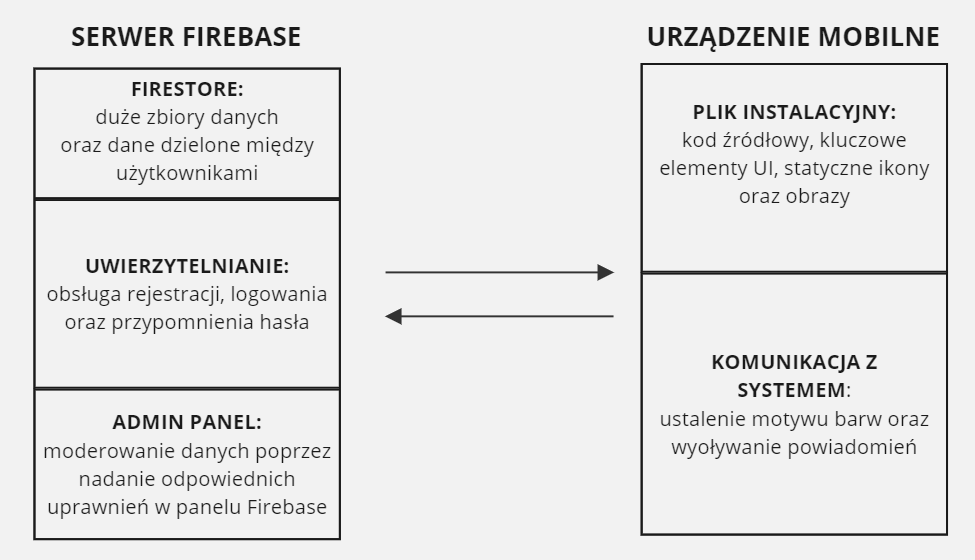
\includegraphics[width=\textwidth]{img/architektura.png}
    \caption{Architektura systemu wraz z funkcjami oraz zawartością poszczególnych elementów}
    \label{architektura}
\end{figure}